\documentclass{standalone}
\usepackage{tikz}
\begin{document}
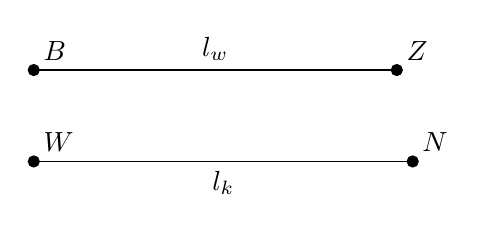
\begin{tikzpicture}[scale=1.0]
  \filldraw (0.0, 0.0) circle (2pt) node[above right] {$B$};
  \filldraw (4.6104, 0.0) circle (2pt) node[above right] {$Z$};
  \filldraw (0.0, -1.1609) circle (2pt) node[above right] {$W$};
  \filldraw (4.8124, -1.1609) circle (2pt) node[above right] {$N$};
  \draw (0.0, 0.0) -- (4.6104, 0.0) node[midway, above] {$l_w$};
  \draw (0.0, -1.1609) -- (4.8124, -1.1609) node[midway, below] {$l_k$};
\end{tikzpicture}
\end{document}